\section{Neural Network}

\begin{wrapfigure}{r}{0.4\textwidth}
  \centering
  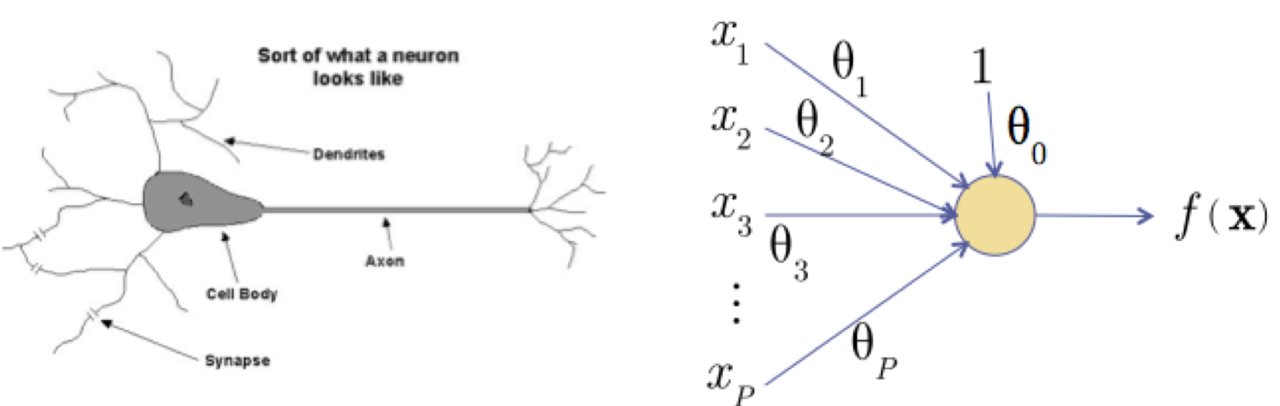
\includegraphics[width=0.38\textwidth]{img/Image.png}
\end{wrapfigure}
Neurons accept information from multiple inputs and transmit information to other neurons.

The idea is to multiply inputs by weights along edges and apply some function to the set of inputs at each node. The inputs are continuous numbers, and a neuron can receive many different signals. We combine this information in a certain way and pass it to the next neuron or emit it as output.

\textbf{Neural Networks} can learn from examples, are universal approximators, can deal with noisy and/or incomplete data, and can handle both continuous and discrete data.

\subsection{Artificial Neurons}
\textbf{Artificial Neural Networks (ANN)} are made up of several \textbf{nodes} (also called \textit{artificial neurons}, or \textit{units}) connected in a net capable of solving AI problems. The single units work and communicate with each other to learn a certain function. The main ideas that these models are based on are:

\begin{itemize}
    \item \textbf{Strength reinforcement}: stimuli ``reinforce'' the weights;
    \item \textbf{Plasticity}: the nervous system is highly capable of adapting.
\end{itemize}

Each neuron $i$ has a number of \textbf{inputs} coming from external sources or other units, and corresponding \textbf{weights}: the free parameters modified during the learning phase. A weight represents the strength of the connection from unit $j$ to unit $i$; the higher the value, the stronger the connection, while its sign tells us whether the connection is positive or negative.

\begin{wrapfigure}{r}{0.25\linewidth}
    \centering
    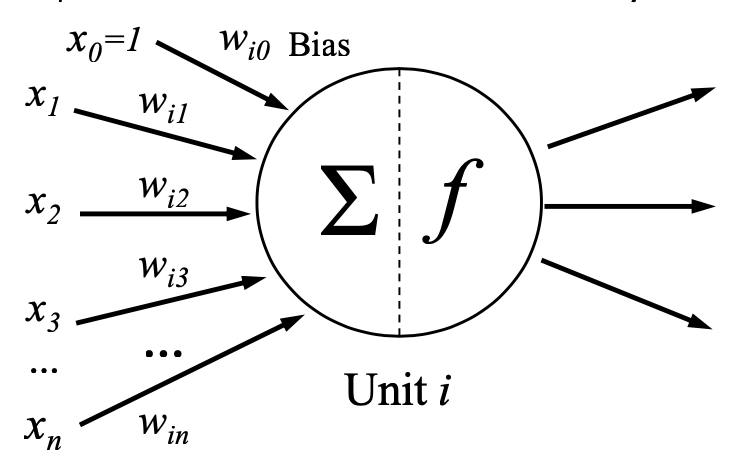
\includegraphics[width=\linewidth]{img/Neuron.png}
\end{wrapfigure}

The model is an assembly of interconnected nodes and weighted links. The output node sums each of its input values according to the weights of its links and compares them against some threshold $t$ (called bias $b$).


\begin{equation*}
    \begin{cases}
        b=\theta_{i0}x_0\,\, with\,\, x_0=1 & b \text{ bias}\\
        net_i(x) = \sum_{j=0}^n w_{ij} x_j & net_i \text{ net input}, w_{ij}\text{ weight with $j$ as input}\\
        o_i(x) = f(net_i(x))& f \text{ activator function}
    \end{cases}
\end{equation*}

\textit{Note:} $w_{ij}$ is the weight of the edge $j\to i$; sometimes the opposite notation is used.

The \textbf{simple linear neuron} has $y=h_\theta(x)=\sigma(\theta^Tx)$ as activation function, where $\sigma(a) = a$.
This approach has no imbalance toward any class, and it always returns the identity (\textit{useless}).

A more useful choice is the \textbf{logistic neuron}, which uses $y=h_\theta(x)=\sigma(\theta^Tx)$ as activation function, where
    \begin{equation}
    \sigma(a)=\dfrac{1}{1+e^{-a}}        
    \end{equation}


\subsubsection{Perceptrons}
A perceptron is a type of artificial neuron used for \textbf{binary classification}. It consists of an input layer $x=(x_1,\dots,x_n)$, a set of weights $w_i$, a bias term $b$, and an activation function $\sigma(z)$. The perceptron computes a weighted sum ($z$), and the output is determined using a step activation function ($\sigma(z)$).
\begin{equation*}
    z = \theta^T x = \sum_{i=1}^{n} w_i x_i + b
\qquad \sigma(z)=
        \begin{cases}
       +1 \,,\; z\geq 0\\
       -1 \,,\; z < 0
    \end{cases}
\end{equation*}

Since the perceptron consists of only an input layer and an output node, it is classified as a \textbf{single-layer network}. It is limited to linearly separable problems but serves as the foundation for more complex neural architectures.

\paragraph{Logical Operations with Perceptrons}
This model can represent the boolean functions AND and OR using a single neuron (linear problems). Each neuron has two inputs plus a bias ($w_0$). Both problems are linearly separable, so if we plot the inputs on a plane, we can draw a single line that separates all inputs producing a 0 from all those producing a 1.

\begin{center}
    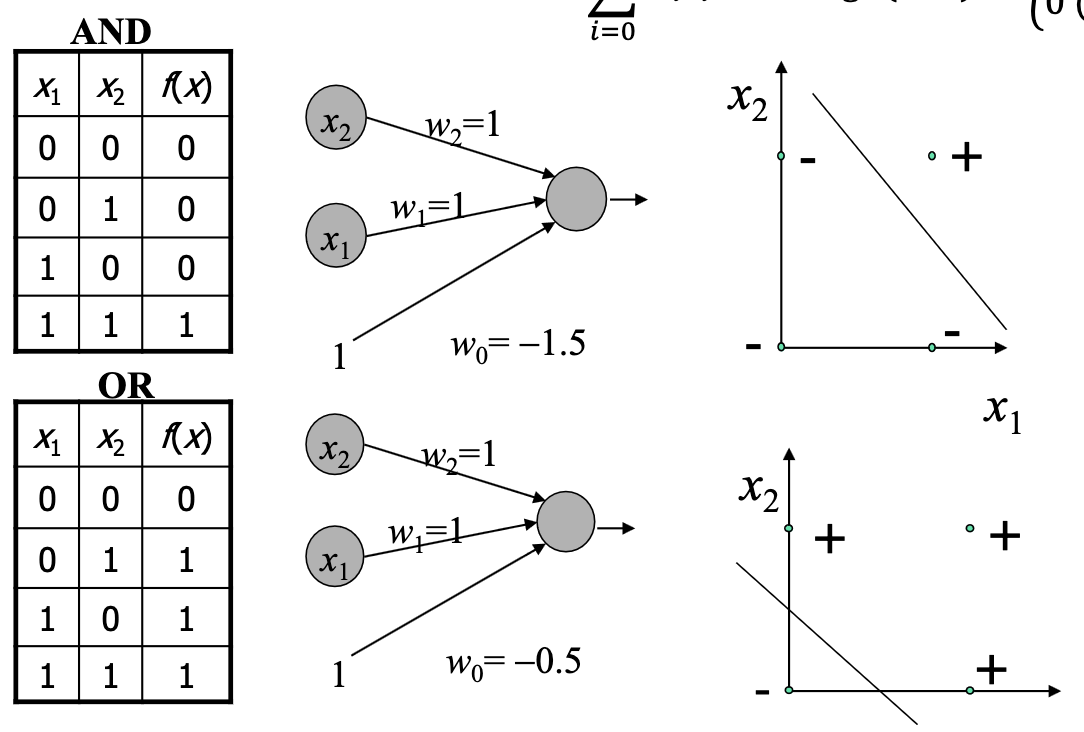
\includegraphics[width=0.5\linewidth]{img/boolean perceptron.png}
\end{center}
For non-linearly separable problems the perceptron fails, because no linear hyperplane can separate the data perfectly. One example is the XOR operator, for which a single neuron does not suffice. The solution is a two-layer network. We can rewrite the operation as follows:

\begin{equation*}
    x_1 \oplus x_2 = x_1 \cdot \bar{x_2} + \bar{x_1} \cdot x_2 \Longrightarrow
    x_1 \oplus x_2 = \bar{h_1} \cdot h_2
\end{equation*}
The XOR operation is moved to a new space that represents the problem as linearly separable:
\begin{center}
    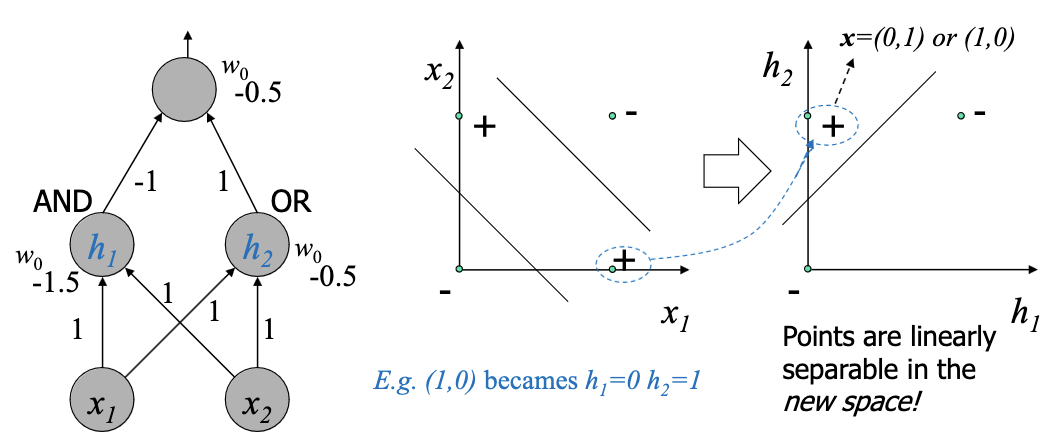
\includegraphics[width=0.55\linewidth]{img/xor perceptron.png}
\end{center}
This kind of composition can perform more complex tasks, extending the network to many layers of abstraction. In a neural network, this internal representation can be learned.
\subsection{Learning Algorithms for One-Unit Models}

There are two kinds of learning algorithms:
\begin{itemize}
    \item \textbf{Adaline (Adaptive Linear Neuron)}: linear unit during training, can use LMS with either the SVD or the gradient descent algorithm. This approach generalizes to multi-layer perceptron networks.

    \item \textbf{Perceptron}: non-linear unit during training, with hard limit or threshold activation function. Can only be used for classification.
\end{itemize}

\subsubsection{Perceptron Learning Algorithm}

The perceptron algorithm minimizes misclassified patterns by finding $w$ such that $sign(w^Tx) = d$. It updates the weights iteratively for each training example:

\begin{itemize}
    \item Initialize weights randomly or to small values.
    \item Choose a learning rate $\eta$.
    \item For each training pair $(x, d)$:
    \begin{itemize}
        \item Compute $out = sign(w^T x)$.
        \item If $out \neq d$, update weights:
        \begin{equation*}
            w_j^{(k+1)} = w_j^{(k)} + \eta (d - out) x_j
        \end{equation*}
    \end{itemize}
\end{itemize}

Geometrically, this shifts $w$ in the direction of $x$ when $x$ is misclassified.
The learning rate $\eta \in (0,1)$ controls the step size: a small $\eta$ leads to slow convergence, a large $\eta$ risks overshooting. An adaptive $\eta$ can start high and decrease over iterations.

\paragraph{Least Mean Squares and Perceptron: Learning Algorithm Differences}
The perceptron and LMS are similar in that both update $w$ using a correction term $\delta$ multiplied by the learning rate $\eta$. The key difference lies in $\delta$:
\begin{itemize}
    \item LMS: $\delta = (d - w^Tx)$
    \item Perceptron: $\delta = (d - sign(w^Tx))$
\end{itemize}

Despite this similarity, the two algorithms differ in important ways:
\begin{itemize}
    \item LMS does not directly minimize misclassification, as it updates weights for both correct and incorrect classifications.
    \item The perceptron algorithm always converges to a perfect classifier for linearly separable problems, while LMS converges asymptotically, even for non-linearly separable cases.
    \item LMS extends naturally to neural networks using gradient-based optimization, whereas the perceptron learning algorithm is harder to generalize.
\end{itemize}

\subsection{Activation Functions}
Activation functions can be:
\begin{itemize}
    \item \textbf{linear}: no non-linear transformations.
    \item \textbf{threshold-based}: as in perceptron/LTU.
    \item \textbf{non-linear}: as the sigmoid function, which is continuous, differentiable, and bounded in \([0,1]\).
\end{itemize}\begin{itemize}[leftmargin=*, nosep]
    \item \textbf{Sigmoid (logistic):}
    \begin{align}
        f_{\sigma}(x) &= \frac{1}{1+e^{-ax}} \quad \text{where } f_{\sigma}(x) \in [0,1] \\
        \frac{d f_{\sigma}(x)}{dx} &= a f_{\sigma}(x)(1 - f_{\sigma}(x))
    \end{align}
    
    \item \textbf{Hyperbolic tangent:}
    \begin{align}
        f_{\tanh}(x) &= 2f_{\sigma}(x) - 1 \quad \text{where } f_{\tanh}(x) \in [-1,1] \\
        \frac{d f_{\tanh}(x)}{dx} &= \frac{a}{2}\left(1 - f_{\tanh}(x)^2\right)
    \end{align}
    
    \item \textbf{Radial Basis Function (RBF):}
    \begin{equation}
        f(x) = e^{-ax^2}
    \end{equation}
    
    \item \textbf{ReLU (Rectified Linear Unit):}
    \begin{equation}
        f(x) =
        \begin{cases}
            0 & x < 0 \\
            x & x \geq 0
        \end{cases}
    \end{equation}
    
    \item \textbf{Softplus:}
    \begin{equation}
        f(x) = \ln(1+e^x)
    \end{equation}
\end{itemize}
Non-linear activation functions introduce complexity into the model, enabling neural networks to learn more sophisticated patterns.

\subsubsection{LMS With a Sigmoidal Function}
Since the sigmoid function is differentiable, we can derive an LMS algorithm by computing the gradient of the mean squared loss, as we did for linear units. The neuron's output is:

\begin{equation*}
    out(x) = f_{\sigma}(x^Tw)
\end{equation*}

The goal is to minimize the residual sum of squares:

\begin{equation*}
    w = \arg\min_w E(w) = \sum_p (d_p - f_{\sigma}(x_p^Tw))^2
\end{equation*}

Gradient descent follows the updated delta rule:

\begin{equation*}
    w_{new} = w + \eta \delta_p x_p, \quad \delta_p = (d_p - out(x_p)) f'_{\sigma}
\end{equation*}

The slope parameter \(a\) affects the gradient step. The derivative \( f' \) is maximized for net inputs near zero and minimized in \textbf{saturated cases}, where \( f \) asymptotically approaches 0 or 1.



\subsection{Multi-Layer Perceptrons (MLP)}

An \textbf{MLP} can be seen in two ways: either as a network of units, or as a flexible function. As a network, an MLP contains a number of units connected by \textbf{weighted links}. The units are organized in layers: the first layer, which loads the input, is the \textbf{input layer}; the layer that produces the final output is the \textbf{output layer}; all the layers in between are \textbf{hidden layers}. We use the following notation for networks:

\begin{itemize}
    \item the index $t$ denotes a generic unit, while $k$ denotes an output unit;

    \item the index $u$ denotes a generic input component;

    \item $x$ is a generic input from an external source (when it is an input vector) or from another unit;

    \item once $x$ is loaded in the input layer, the notation $o$ can denote both inputs and hidden-layer inputs, so in the network the input to each unit $t$ from any source $u$ is written $o_u$.
\end{itemize}
As a flexible function, the MLP can be written in the following form:
\begin{equation}
    h(x) = f_k(\sum_j w_{kj} f_j (\sum_i w_{ji} f_i(\dots)))  \qquad f_k \text{ sigmoid activation function}
\end{equation}

The \textbf{architecture} of a NN defines the topology of the connections between units. A \textbf{feedforward architecture} describes a network that operates as follows. For each input pattern $x$, do:

\begin{itemize}
    \item load the input in the input layer;
    \item compute the output of all the units in the first hidden layer;
    \item compute the output of all the units in the second hidden layer;
    \item ...
    \item compute the output of all the units in the output layer;
    \item compute the error (delta) at the output level.
\end{itemize}
A \textbf{recurrent architecture} describes a network with feedback loops, which let the output of units flow ``back'' through the network toward units in previous layers.

\subsection{Hypothesis Space of a Neural Network}

The hypothesis space of a neural network encompasses all functions representable by assigning weights to a given architecture. These models can address both regression and classification tasks, using linear or sigmoidal output functions respectively. They can also implement multi-regression and multi-class classification through multiple output units.

When viewing a neural network as a function:
\begin{equation*}
    h(x) = f_k\left(\sum_j w_{kj} f_j \left(\sum_i w_{ji} f_i(\ldots)\right)\right) \, ,
\end{equation*}
each unit $f_j$ can be considered an independent component, analogous to basis functions in Linear Basis Expansion. However, $h(x)$ is non-linear in the parameters $w$. We can reformulate this as:
\begin{equation*}
    h(x) = f_k\left(\sum_j w_{kj} f_j \left(\sum_i w_{ji} x_i\right)\right) = f\left(\sum_j w_j \phi_j(x,w)\right)
\end{equation*}

The key distinction from Linear Basis Expansion is that the basis functions $\phi$ are adapted to the data by optimizing the weights $w$.

\begin{theorem}[Universal Approximation]
A single hidden-layer network with logistic activation functions can approximate any continuous function given sufficient units. Similarly, a multilayer perceptron can approximate any input-output mapping with enough hidden units. However, this theorem neither specifies the learning algorithm nor the required number of units.
\end{theorem}

Two fundamental questions arise: how to train neural networks and how to select their architecture. The network's expressive power depends on both the number of units and the architectural design. The number of parameters $w$ (proportional to the number of units) affects its capacity, and smaller weights reduce the VC-dimension.

The number of layers matters too. While the universal approximation theorem guarantees that a single layer suffices, the required number of units may be impractically large. To keep complexity manageable, networks are usually structured with multiple layers, each holding a reasonable number of units.

\subsection{Backpropagation Learning Algorithm}

The neural network learning algorithm follows the Least Mean Squares approach, adapting the parameters $w$ to best approximate the target function by minimizing the error (loss) function over the training set. With multiple units spread across layers, the algorithm must determine each hidden unit's contribution to the error.

The \textbf{loading problem} asks whether there exists a set of weights making the network consistent with the training examples. This problem is NP-complete: while training can be performed in reasonable time, optimal solutions cannot be guaranteed.

Backpropagation extends gradient descent to multilayer perceptron networks, requiring:
\begin{itemize}
    \item A differentiable loss function
    \item Differentiable activation functions
    \item Clear information flow through the network
\end{itemize}

The goal is to compute the gradient of the error function with respect to weights $w$. Backpropagation offers several advantages:
\begin{itemize}
    \item Simplicity due to the model's compositional form
    \item Ability to track local quantities within each unit
    \item Computational efficiency, with complexity of $O(\#W)$ rather than $O(\#W^2)$
\end{itemize}

\subsection{Issues in Training Neural Networks}

The resulting model is often over-parameterized; on top of that, the optimization problem is no longer convex, and is potentially unstable.


\subsubsection{Hyperparameters}

\paragraph{Starting Values}

Weights are typically initialized randomly near 0 to avoid issues such as a null weight vector, excessively high values, or identical components. The \textbf{fan-in} (number of inputs to a hidden unit) matters, since a large fan-in may cause gradients to vanish during backpropagation, hurting training.

For MLP with backpropagation, the gradient is calculated as:
\begin{equation*}
    - \dfrac{\partial E(w)}{\partial w_{tu}} = \sum_{p=1}^l \delta_{p,t} o_{p,u} \quad \text{(batch)}
\end{equation*}
\begin{equation*}
    - \dfrac{\partial E(w)}{\partial w_{tu}} = \delta_{p,t} o_{p,u} \quad \text{(online)}
\end{equation*}

Basic SGD is efficient, though its performance depends on the number of training examples and epochs. Other heuristic methods include Quick-prop, which finds the minima of a local convex function, and R-prop, which uses only the gradient sign.

\textbf{Second-order methods} estimate the curvature of the objective function to improve descent, for example Newton's methods or Hessian-free approaches (conjugate gradients, quasi-Newton). They are less common for neural network training, because they are sensitive to saddle points, which grow exponentially in number in high-dimensional spaces. Gradient descent, by contrast, escapes saddle points more easily. The long training path of gradient descent may stem from other factors that are still under study.

In practice, basic methods are generally sufficient when applied correctly, with the main focus on validation rather than training set optimization.

\paragraph{Learning Rate}

A higher $\eta$ speeds up descent but increases instability, while a lower $\eta$ slows it down but keeps it stable. To monitor the model's behavior and tune $\eta$, we use a \textbf{learning curve}, which plots the error against the epochs.

\begin{figure}[ht]
    \centering
    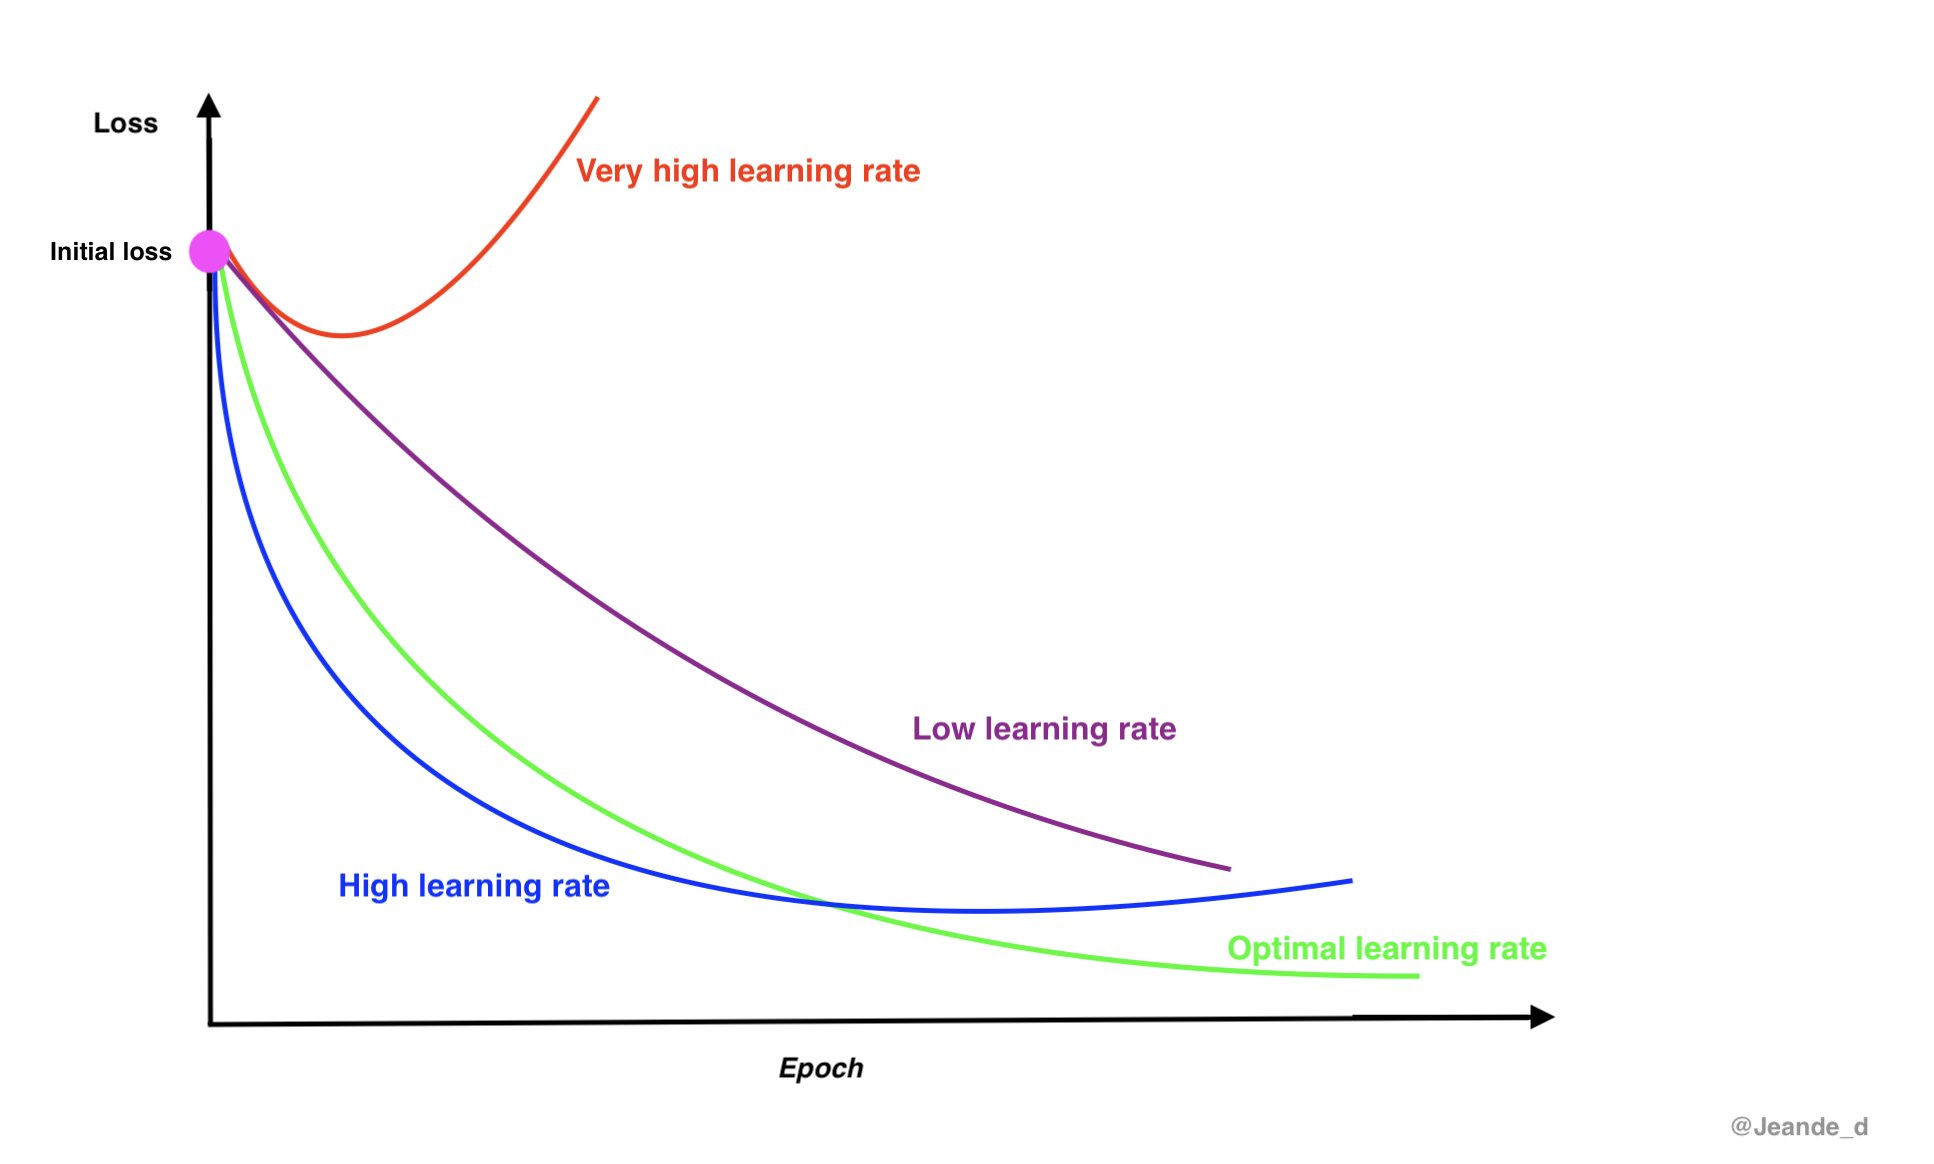
\includegraphics[width=0.5\linewidth]{img/Learning curve and eta.png}
\end{figure}

A practical approach is to consider the mean gradient over an epoch, ensuring uniformity across input data. In LMS, dividing by $l$ is equivalent to using $\eta/l$. To improve learning rate selection, the following methods can be applied:

\begin{itemize}
    \item \textbf{Momentum}: Adds inertia to weight updates:
    \begin{equation*}
        \Delta w = - \eta \dfrac{\partial E(w)}{\partial w} + \alpha \Delta w_{old} \qquad \alpha\in (0,1)
    \end{equation*}
    This \textit{heavy ball method} accelerates training on plateaus and dampens oscillations, allowing a higher $\eta$. A variant, \textbf{Nesterov momentum}, applies the momentum before evaluating the gradient, improving convergence in batch mode.

    \item \textbf{Variable learning rate}: Starts high and decreases. In minibatch training, the gradient never reaches 0 near a minimum, so a fixed $\eta$ is suboptimal. We linearly decay $\eta$ until iteration $\tau$:
    \begin{equation*}
        \eta_s = (1-\alpha)\eta_0 + \alpha \eta_{\tau} \qquad \eta_{\tau} \approx 1\% \text{ of } \eta_0
    \end{equation*}

    \item \textbf{Adaptive learning rates}: Automatically adjust $\eta$ during training, reducing hyperparameter tuning. Popular methods include AdaGrad, RMSProp, and Adam, often combined with momentum.

    \item \textbf{Layer-wise adjustments}: Higher $\eta$ for deep layers or units with fewer input connections.
\end{itemize}

\paragraph{Number of Units}

The number of units determines the network's complexity. This is a model selection issue, typically handled through cross-validation. Too few units cause underfitting, while too many can lead to overfitting, though regularization can mitigate this. Two main approaches exist:

\begin{itemize}
    \item \textbf{Constructive}: Start with a small network and add units as needed.
    \item \textbf{Pruning}: Begin with a large network and remove unnecessary units/weights.
\end{itemize}

A well-known constructive approach is the \textbf{Cascade Correlation (CC)} algorithm, which incrementally builds the network while learning both weights and topology. This algorithm alternates between minimizing the error function and maximizing the correlation (covariance of the new unit's output with the residual error). Hidden units progressively reduce residual error.

\begin{algorithm}
\caption{Cascade Correlation Algorithm}
\begin{algorithmic}[1]
    \State Train an initial network $N_0$ (no hidden units) and compute error.
    \If{$N_0$ does not solve the problem}
        \State Set $i = 1$.
        \Repeat 
            \State Add a new unit to form $N_i$.
            \State Train the unit to maximize correlation with the residual error of $N_{i-1}$.
            \State Freeze its weights and retrain the remaining units.
            \State Compute error of $N_i$.
            \State Increment $i$.
        \Until{error $\leq$ threshold.}
    \EndIf
\end{algorithmic}
\end{algorithm}

\subsubsection{Multiple Minima}

The loss function is non-convex, leading to multiple minima and maxima. The final outcome depends heavily on the initial weights. A practical approach runs several random trials, computes the mean error, and assesses the variance. We can then pick the best solution by the lowest or median validation error, or by the mean output.

Reaching a local minimum with high error is not a major problem, since we can restart training if needed. The goal is not the global minimum but a sufficiently good local one, because we optimize $R_{emp}$, not $R$. Rather than stopping at a zero-gradient point, it may be preferable to halt when the gradient is small enough.

Another key factor is that neural network training expands the hypothesis space and raises the VC-dim. As the VC-dim grows, $R_{emp}$ decreases, but overfitting becomes more likely. So stopping before the minimum may yield a better approximation of the target function.

\subsubsection{Stopping Criteria}

A basic stopping criterion monitors the error (mean or max $E$), but setting a proper tolerance threshold can be hard. Instead, we can stop once the error improvement (e.g. $<0.1\%$) or the weight changes (e.g. $\|\nabla E\| < \eta$) become negligible.

Stopping at a fixed number of steps is ineffective: too few steps cause underfitting, while too many risk overfitting. In K-Fold cross-validation, the optimal number of epochs varies per fold. A common approach treats the number of epochs as a hyperparameter and selects the mean across folds. Retraining on the full dataset, however, may shift the optimal stopping point and lead to underfitting.


\subsubsection{Overfitting and Regularization}

As noted, the global minimizer of $R_{emp}$ often leads to overfitting. Controlling complexity requires regularization, either through a penalty term or early stopping. Cross-validation helps find the best trade-off.

Neural network training starts with small random weights, keeping the VC-dim low. As training progresses, hidden units saturate, raising the number of free parameters and the VC-dim. When should we stop?

\begin{itemize}
    \item \textbf{Early stopping}: Using a validation set to determine the optimal stopping point. Since the number of effective parameters grows during training, stopping limits complexity.
    
    \item \textbf{Regularization}: Adding a penalty term based on Tikhonov theory:
    \begin{equation*}
        Loss(w) = \sum_p (d_p - o(x_p))^2 + \lambda\|w\|^2
    \end{equation*}
    This introduces weight decay, as gradient updates include $- \lambda w$, reducing weights even when $\Delta w = 0$. The regularization parameter $\lambda$ is chosen during model selection.

    \item \textbf{Pruning methods}: Discussed later.
\end{itemize}

Regularization affects the training loss but not the evaluation error, since it only controls model complexity. Contrary to common belief, it does not improve convergence stability. Early stopping (empirical) requires a validation set, while regularization (principled) keeps the validation and training curves aligned.

The bias $w_0$ is often excluded from regularization to stay independent of target shift or scaling. When it is included, it needs a separate regularization term.

\paragraph{Momentum and Weight Decay Together}

Combining both, the weight update is:
\begin{equation*}
    \Delta w = -\eta \dfrac{\partial Loss(w)}{\partial w} + \alpha \Delta w_{old} \doteq \eta \delta o - \lambda w + \alpha \Delta w_{old}
\end{equation*}
A common alternative formulation keeps hyperparameters separate:
\begin{equation*}
    \Delta w = \eta \delta o + \alpha \Delta w_{old}
\end{equation*}
\begin{equation*}
    w_{new} = w + \Delta w - \lambda w
\end{equation*}

\subsubsection{Input Scaling and Output Representation}
Preprocessing has a strong effect on neural network training. Data should be normalized via:

\begin{itemize}
    \item \textbf{Standardization}: Each feature is transformed to have mean 0 and standard deviation 1.
    \item \textbf{Rescaling}: Values are restricted to [0,1].
\end{itemize}

For regression, outputs are linear units; for classification, outputs can be:

\begin{itemize}
    \item A single binary unit.
    \item Multiple binary units with a sigmoid threshold, rejection zone, or 1-to-K encoding.
\end{itemize}

The symmetric logistic function often speeds up learning. To prevent asymptotic convergence, we use labels of 0.9 and 0.1 instead of 1 and 0 (or -0.9 instead of -1 for tanh). The target range must align with the unit output range.

For 0/1 classification, Softmax is common:
\begin{equation*}
    o_k(x) = \dfrac{e^{net_k}}{\sum_{j=1}^K e^{net_j}}
\end{equation*}
Cross-entropy loss is often used for optimization:
\begin{equation*}
   E(w) = - \sum_{i \in TR} \left[ d_i \log (out(x_i)) + (1-d_i) \log(1-out(x_i)) \right]
\end{equation*}


\paragraph{When to Consider Neural Networks}
\begin{itemize}
    \item the input is high-dimensional, discrete or real-valued, for both regression and classification tasks;

    \item the dataset may contain noise;

    \item the form of the target function is unknown;

    \item human readability of the output is not important;

    \item training time is not a constraint;

    \item the computation of the output itself has to be fast.
\end{itemize}